%=================
\chapter{Sprint I}
%=================


%------------------------
\section{Sprint Planning}
%------------------------
In our first sprint we will implement basic and fundamental parts of the
utility. Based on our preliminary studies, we have decided what preprocessor
and parser to use, so the task is to make this work together and achieve the
desired functionality.

\subsection{Duration}
%--------------------
Sprint 1 started September 14th, and lasted until September 27th. To avoid
misunderstandings between our developers and the customer, we will have weekly
meetings to show what we have accomplished and discuss further development. 

\subsection{Sprint Goal}
%-----------------------
The overall goal of the first sprint is to create a preliminary design and
implement the core of the application. It will be possible to run it to
generate Lua dissectors which can be used by Wireshark users. The first
version will contain only the basic dissector generating features, i.e.
parsing C structs with basic data types as members. Also, some of the
preprocessing capabilities will be implemented, such as handling \#include
directives. Basic support for configuration will be added.

\subsection{Back Log}
The first sprint we will implement eight requirements. Table
\ref{tab:sp1_req7a}-\ref{tab:sp1_req2d}  list each requirement with a time
estimate. \autoref{tab:sprint1req} is the sprint backlog for the first phase.
\autoref{tab:sprint1time} is the time table for the first phase.

\begin{table}[!ht] \small \center
\caption{Sprint 1 Requirement FR6-A\label{tab:sp1_req7a}}
\begin{tabular}{l l c}
	\toprule
	Requirement & Task & Hours \\
	\midrule
	\multirow{4}{5cm}{Command line shall support parameter for C header file} & Design & 1 \\
	& Implementation & 2 \\
	& Testing & 2 \\
	& Documentation & 4 \\
	\bottomrule
\end{tabular}
\end{table}

\begin{table}[!ht] \small \center
\caption{Sprint 1 Requirement FR1-A\label{tab:sp1_req1a}}
\begin{tabular}{l l c}
	\toprule
	Requirement & Task & Hours \\
	\midrule
	\multirow{4}{5cm}{The utility must support the following basic data types: int, float, char and boolean} & Design & 4 \\
	& Implementation & 8 \\
	& Testing & 8 \\
	& Documentation & 4 \\
	\bottomrule
\end{tabular}
\end{table}

\begin{table}[!ht] \small \center
\caption{Sprint 1 Requirement FR2-A\label{tab:sp1_req2a}}
\begin{tabular}{l l c}
	\toprule
	Requirement & Task & Hours \\
	\midrule
	\multirow{4}{5cm}{The dissector shall be able to display simple structs} & Design & 4 \\
	& Implementation & 8 \\
	& Testing & 8 \\
	& Documentation & 8 \\
	\bottomrule
\end{tabular}
\end{table}

\begin{table}[!ht] \small \center
\caption{Sprint 1 Requirement FR3-A\label{tab:sp1_req3a}}
\begin{tabular}{l l c}
	\toprule
	Requirement & Task & Hours \\
	\midrule
	\multirow{4}{5cm}{The utility shall support \#include} & Design & 2 \\
	& Implementation & 2 \\
	& Testing & 2 \\
	& Documentation & 2 \\
	\bottomrule
\end{tabular}
\end{table}

\begin{table}[!ht] \small \center
\caption{Sprint 1 Requirement FR3-B\label{tab:sp1_req3b}}
\begin{tabular}{l l c}
	\toprule
	Requirement & Task & Hours \\
	\midrule
	\multirow{4}{5cm}{The utility shall support \#define and \#if} & Design & 1 \\
	& Implementation & 2 \\
	& Testing & 6 \\
	& Documentation & 2 \\
	\bottomrule
\end{tabular}
\end{table}

\begin{table}[!ht] \small \center
\caption{Sprint 1 Requirement FR6-B\label{tab:sp1_req7b}}
\begin{tabular}{l l c}
	\toprule
	Requirement & Task & Hours \\
	\midrule
	\multirow{4}{5cm}{Command line shall support parameter for configuration file} & Design & 8 \\
	& Implementation & 8 \\
	& Testing & 8 \\
	& Documentation & 4 \\
	\bottomrule
\end{tabular}
\end{table}

\begin{table}[!ht] \small \center
\caption{Sprint 1 Requirement FR4-A\label{tab:sp1_req4a}}
\begin{tabular}{l l c}
	\toprule
	Requirement & Task & Hours \\
	\midrule
	\multirow{4}{5cm}{Configuration must support valid ranges for struct members} & Design & 6 \\
	& Implementation & 8 \\
	& Testing & 8 \\
	& Documentation & 8 \\
	\bottomrule
\end{tabular}
\end{table}

\begin{table}[!ht] \small \center
\caption{Sprint 1 Requirement FR2-D\label{tab:sp1_req2d}}
\begin{tabular}{l l c}
	\toprule
	Requirement & Task & Hours \\
	\midrule
	\multirow{4}{5cm}{The dissector shall be able to recognize invalid values for a struct member} & Design & 4 \\
	& Implementation & 6 \\
	& Testing & 8 \\
	& Documentation & 4 \\
	\bottomrule
\end{tabular}
\end{table}

\begin{table}[!ht] \small \center
\caption{Sprint 1 Requirements\label{tab:sprint1req}}
\begin{tabularx}{\textwidth}{l l X c c}
	\toprule
	& & & \multicolumn{2}{c}{Hours} \\
	\cmidrule(r){4-5}
	\# & Req. & Description & Est. & Act. \\
	\midrule
	1 & FR6-A & Command line shall support parameter for C header file & 9 & 9\\
	\addlinespace
	2 & FR1-A & Support basic data types: int, float, char, boolean & 24 & 21\\
	\addlinespace
	3 & FR2-A & The dissector shall be able to display simple structs & 28 & 25\\
	\addlinespace
	4 & FR3-A & The utility shall support \#include & 8 & 2\\
	\addlinespace
	5 & FR3-B & The utility shall support \#define and \#if & 11 & 3\\	
	\addlinespace
	6 & FR6-B & Command line shall support paramter for configuration file & 28 & 8\\
	\addlinespace
	7 & FR4-A & Support valid ranges for struct members & 30 & 15 \\
	\addlinespace
	8 & FR2-D & Recognize invalid values for a struct member & 22 & 15\\
	\midrule
	& & Total: & 160 & 98\\
	\bottomrule
\end{tabularx}
\end{table}

\begin{table}[!ht] \small \center
\caption{Sprint 1 Timetable\label{tab:sprint1time}}
\begin{tabularx}{\textwidth}{X c c}
	\toprule
	& \multicolumn{2}{c}{Hours} \\
	\cmidrule(r){2-3}
	Description & Est. & Act. \\
	\midrule
	Design & 30 & 10\\
	\addlinespace
	Implementation & 44 & 65 \\
	\addlinespace
	Testing & 50 & 20\\
	\addlinespace
	Documentation & 36 & 3\\
	\midrule
	Total: & 160 & 98 \\
	\bottomrule
\end{tabularx}
\end{table}


%----------------------
\section{System Design}
%----------------------
This section introduces the design goals we decided on, the preliminary overall
design, and the final system design after the first sprint. In
\autoref{sec:sp1:impl} we describe how our implementation works and are to be
used.

\subsection{Design Goals}
%------------------------
To help guide the design and the implementation we tried to follow these
goals and guidelines:
\begin{itemize}
	\item Smart data structures and dumb code works a lot better than the other
		way around\cite{Raymond1999}!
	\item Clear and clean separation of the front-end and the back-end so in the
		future other parsers can be used to generate dissectors.
	\item Try to be pythonic, follow
		PEP8\footnote{Style Guide for Python Code: \url{http://www.python.org/dev/peps/pep-0008/}} and
		PEP20\footnote{The Zen of Python \url{http://www.python.org/dev/peps/pep-0020/}}.
	\item Now is better than never. Don't be afraid to write stupid or ugly
		code, we can always fix it later.
	\item The first version is never perfect, so don't wait until its perfect
		before you commit. Commit often!
\end{itemize}

\subsection{Preliminary Design}
%------------------------------
The following is a description of the preliminary design we had for our
utility. We split our program into the several parts, described in the
following paragraphs, their relationship is explained in
\autoref{fig:sp1:design}.

\begin{figure}[!htb]
	\center
	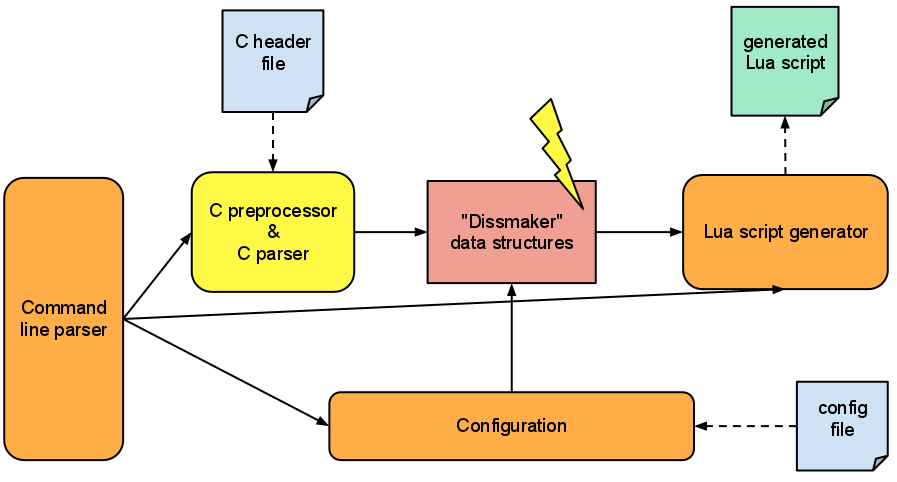
\includegraphics[width=\textwidth]{./sprints/img/design}
	\caption{Overall design\label{fig:sp1:design}}
\end{figure}

\paragraph{Command line interface}
The command line interface is where the user inputs which header files and
configuration files he wants the utility to use. This module needs to ask
the configuration to parse config files, and then ask the front-end to parse C
files. It should finally ask the back-end to generate Wireshark dissectors
for the given header files. The CLI should be able to accept some additional
arguments like verbose, debug, nocpp and output options.
The argument verbose should print out detailed information,
debug should print out debugging information, and nocpp should
disable the C preprocessor. If the CLI is provided with invalid arguments, 
it should print a message explaining the correct usage.
If the program ran as expected it should output a message informing
the user of the success. 

\paragraph{Configuration}
The configuration should parse the configuration files given
to the command line interface, and from this information modify
the data structures generated by the front-end.

\paragraph{Front-end}
The front-end of the system is the parser, it should parse C files and
look for struct definitions. The struct definitions will be put into a data structure
that the back-end will use when creating the dissectors.

The front-end should use pycparser and PLY libraries for parsing of C files. It should accept C
header files and create an abstract syntax tree, which is traversed
to find struct definitions and their members. The struct definitions and members
are then filled into a suitable data structure.

\paragraph{Data Structures}
The data structures should store the information the back-end needs to generate
Wireshark dissectors. It should have support for protocols and fields in Wireshark.
The data structures should be easily modifiable by the configuration.

\paragraph{Back-end}
The back-end is the part of the system that generates the actual Lua dissectors.
It should use the information in the data structures, that the 
front-end and configuration generates, to create Lua code that can dissect
the header files inputted by the user. 

\subsection{Utility}
%-------------------
Figure \ref{fig:sp1_class} illustrates the current class diagram for our
utility after the end of the first sprint. The csjark module contains the main
method of the utility and is responsible for running the program.
It is in this module we have implemented the functionality for the command line interface.
The utility will typically start off by using cparser to parse the C header file given to
the utility as a command line argument. cparser will then use the config module
to ensure that the parsing is done correctly after the configuration, and then
generate protocols and fields to be used in the csjark module. The csjark
module then generates a Wireshark dissector in Lua code by going through the
protocols and fields generated earlier by the cparser module.

In this sprint we added configuration support for ranges, this was done 
by adding a RangeRule class to the config module. This class specifies how
range rules should be written in the configuration. In the dissector module
we created a RangeField class, that interprets the rules
and recognizes any invalid values when generating the dissectors.
The RangeField class inherits from the Field class.


\begin{figure}[!htb]
	\center
	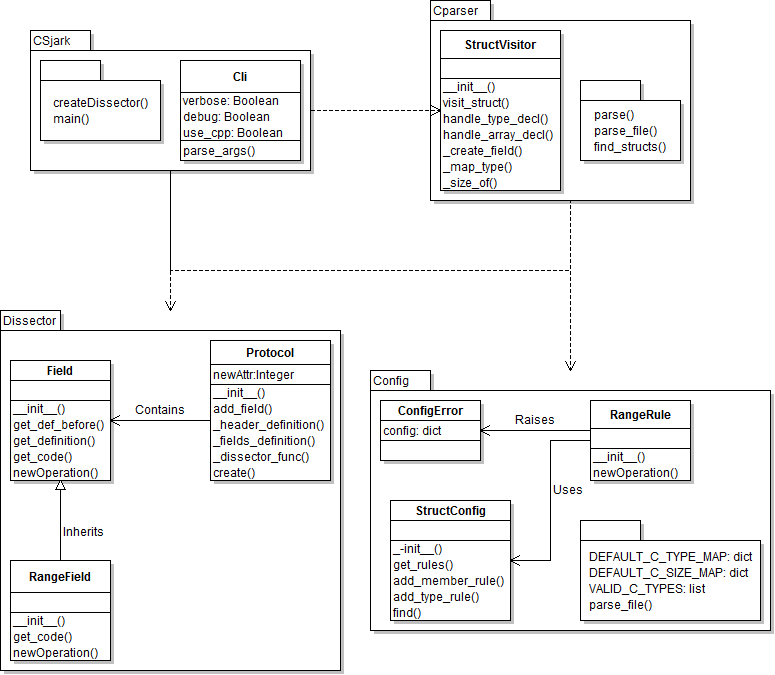
\includegraphics[width=\textwidth]{./sprints/img/class_diagram_s1}
	\caption{Class Diagram\label{fig:sp1_class}}
\end{figure}


%-----------------------
\section{Implementation}
%-----------------------
\label{sec:sp1:impl}
In this sprint we have created a very naive implementation of the utility. It
supports the most basic types of C structs. In addition the utility supports
some very basic configuration. The main reason for the naive implementation, 
was to find out that the libraries that the team had choosen, was suitable for 
the utility and that we had understood the task.

To get a better understanding of how the different requirements were implemented,
look at the user stories for sprint 1 in \autoref{sec:req:stories1}.


\subsection{CLI Support for Header File}
%-------------------
The tool uses a command line interface. The user inputs a C header file to the 
command line, and the program outputs a Wireshark dissector written in Lua. 
Below you can see a \autoref{fig:sp1cmd} that illustrates how the program is 
run. 

\subsection{Support Basic C Data Types}
%-------------------
In this first sprint the focus was to generate dissectors from structs with 
basic datatypes. These datatypes included integers, floats, char, boolean and 
arrays of chars. All different types of integers and floats was also 
implemented in the utility, most of the functionallity was included in the 
pycparser library, and sizes for the different data types was specified in the 
utility.

\subsection{Display Simple Structs}
%-------------------
The dissectors that our utility generates is used to display the packets that 
are captured by wireshark. \autoref{fig:sp1wsstruct} shows an example of a 
packet capture. The example include a struct that is used to test different 
basic data types, for example, signed char, char, short, int, long int, float 
and double.

\begin{figure}[ht]
	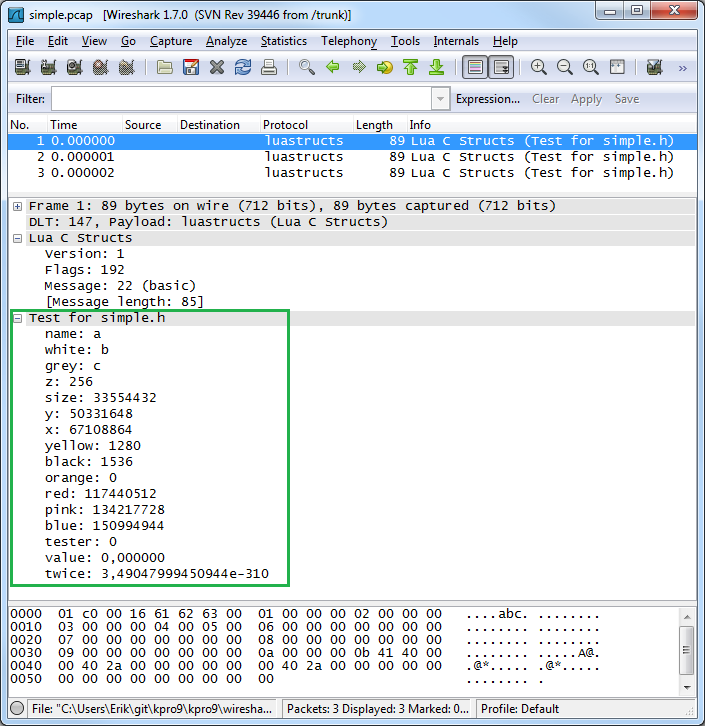
\includegraphics[width=\textwidth]{./sprints/img/wireshark_simple}
	\caption{Command line\label{fig:sp1wsstruct}}
\end{figure}

\subsection{Support \#include}
%-------------------
The preprocessor in C is the first step of compilation. One of the most used 
features in the preprocessor is \#include, which include the content of a file 
in the compilaton. Since the utility reads structs from header-files, it is 
possible that struct member may have been defined in other header-files, 
therefore \#include is a important part of the utility. The preprocessor in 
this utility will replace the \#include-line with the content of the included file.

\subsection{Support \#define and \#if}
%-------------------
These two preprocessor directives are important for our utility. \#define is 
used to define a preprocessor macro that replaces a token with a 
sequence of characters. This can for example be used to define length of 
arrays, define values for enumeration or define a platform. \#if and \#ifdef 
is conditional directives, that the utility will use to check if macros are 
defined, this will be used when the utility are generating dissectors for 
different platforms. The functionallity for these preprocessor directives and 
the other preprocessor directives for C, was implemented by the library we 
use, which is cpp.exe for windows and gcc for mac and linux. 

\subsection{CLI Support for Configuration File}
%-------------------
To be able to parse the configuration file, it is necessary to specify the 
configuration-file in the CLI. An example of this is shown in 
\autoref{fig:sp1cmd}, where a header-file and a config-file is input to the 
utility. The option ''-v'' is specified, which will display the abstract 
syntax tree when the utility has generated the dissector.

\begin{figure}[ht]
	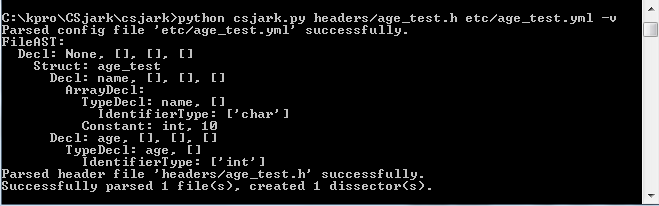
\includegraphics[width=\textwidth]{./sprints/img/cmd_agetest_run}
	\caption{Command line\label{fig:sp1cmd}}
\end{figure}

\subsection{Configuration of Valid Ranges}
%-------------------
We decided to use YAML as our configuration format. In this sprint we have
added support for range specification. A user can specify the ranges of the
members of a struct, from a minimum to a maximum. \autoref{code:rangesconf} 
shows an configuration in YAML for the header-file in \autoref{code:ranges}. 
The configuration specifes that the struct member age, must have a value 
between 0 and 100.  

\lstset{language=C,caption={Configuration of valid ranges},label=code:rangesconf}
\lstinputlisting[language=C]{./sprints/code/ranges.yml}

\lstset{language=C,caption={Header-file for age\_test},label=code:ranges}
\lstinputlisting[language=C]{./sprints/code/ranges.h}

\subsection{Dissector Shall Recognize Invalid Values}
%-------------------
In \autoref{fig:sp1rangerule} you can see how Wireshark displays a member that 
has an invalid range. When a invalid value exist, the dissector will warn the 
user with a message and description, this make it easier for debugging.

\begin{figure}[htb]
	\center
	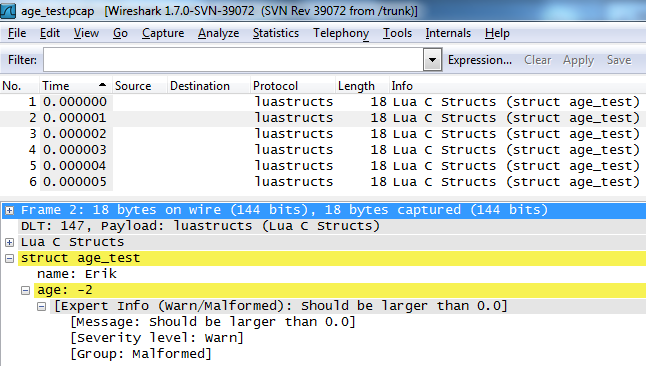
\includegraphics[width=\textwidth]{./sprints/img/wireshark_outofrange}
	\caption{Wireshark dissector\label{fig:sp1rangerule}}
\end{figure}

%-----------------------
\section{Sprint Testing}
%-----------------------
This section introduces the tests preformed during the sprint and their
results.

\subsection{Tests}
%-----------------
During the sprint the team executed a total of 7 tests with names as seen
below. Tests executed:
\begin{itemize}
	\item TID01 - Supporting parameters for c-header file. \autoref{tab:TID01}
	\item TID02 - Supporting basic data types. \autoref{tab:TID02}
	\item TID03 - Displaying simple structs. \autoref{tab:TID03}
	\item TID04 - Supporting c-header files with the \#include directive. \autoref{tab:TID04}
	\item TID05 - Supporting \#define and \#if. \autoref{tab:TID05}
	\item TID06 - Supporting configuration files. \autoref{tab:TID06}
	\item TID07 - Recognizing invalid values. \autoref{tab:TID07}
\end{itemize}

\subsection{Test Results}
%------------------------
These are the results for the tests the team ran for sprint 1 as according to \autoref{tab:testreport} discussed in the test plan.
The test results can be seen in table \ref{tab:sp1_tid01}-\ref{tab:sp1_tid07}.
\begin{table}[!htb] \footnotesize \center
\caption{Supporting parameters for c-header file \label{tab:sp1_tid01}}
\noindent\makebox[\textwidth]{%
\begin{tabularx}{\textwidth}{l X}
	\toprule
	Header & Description \\
	\midrule
	Description & Supporting parameters for c-header file \\
	Tester & Lars Solvoll Tønder \\
	Date & 27.09.2011 \\
	Result & Failure. The LUA-file got created successfully but the user was not informed of the result \\
	\bottomrule
\end{tabularx}}
\end{table}

\begin{table}[!htb] \footnotesize \center
\caption{Supporting basic data types \label{tab:sp1_tid02}}
\noindent\makebox[\textwidth]{%
\begin{tabularx}{\textwidth}{l X}
	\toprule
	Header & Description \\
	\midrule
	Description & Supporting basic data types \\
	Tester & Lars Solvoll Tønder \\
	Date & 27.09.2011 \\
	Result & Failure. The program supports the use of int, float, char and boolean, but did not inform the user of the result\\
	\bottomrule
\end{tabularx}}
\end{table}

\begin{table}[!htb] \footnotesize \center
\caption{Displaying simple structs  \label{tab:sp1_tid03}}
\begin{tabular}{l l}
	\toprule
	Header & Description \\
	\midrule
	Description & Displaying simple structs \\
	Tester & Lars Solvoll Tønder \\
	Date & 27.09.2011 \\
	Result & Success\\
	\bottomrule
\end{tabular}
\end{table}

\begin{table}[!htb] \footnotesize \center
\caption{Supporting c-header files with the \#include directive \label{tab:sp1_tid04}}
\noindent\makebox[\textwidth]{%
\begin{tabularx}{\textwidth}{l X}
	\toprule
	Header & Description \\
	\midrule
	Description &  Supporting c-header files with the \#include directive  \\
	Tester & Lars Solvoll Tønder \\
	Date & 27.09.2011 \\
	Result & Failure. The program supports header files with the \#include directive, but did not inform the user of the result\\
	\bottomrule
\end{tabularx}}
\end{table}

\begin{table}[!htb] \footnotesize \center
\caption{Supporting \#define and \#if \label{tab:sp1_tid05}}
\noindent\makebox[\textwidth]{%
\begin{tabularx}{\textwidth}{l X}
	\toprule
	Header & Description \\
	\midrule
	Description &  Supporting \#define and \#if  \\
	Tester & Lars Solvoll Tønder \\
	Date & 27.09.2011 \\
	Result & Failure. The program supports header files with the \#define and \#if directives, but did not inform the user of the result\\
	\bottomrule
\end{tabularx}}
\end{table}

\begin{table}[!htb] \footnotesize \center
\caption{Supporting configuration files \label{tab:sp1_tid06}}
\noindent\makebox[\textwidth]{%
\begin{tabularx}{\textwidth}{l X}
	\toprule
	Header & Description \\
	\midrule
	Description &  Supporting configuration files  \\
	Tester & Lars Solvoll Tønder \\
	Date & 27.09.2011 \\
	Result & Failure. The program supports the use of configuration files but does not inform the user of any results\\
	\bottomrule
\end{tabularx}}
\end{table}

\begin{table}[!htb] \footnotesize \center
\caption{Recognizing invalid values \label{tab:sp1_tid07}}
\begin{tabular}{l l}
	\toprule
	Header & Description \\
	\midrule
	Description &  Recognizing invalid values  \\
	Tester & Lars Solvoll Tønder \\
	Date & 27.09.2011 \\
	Result & Success\\
	\bottomrule
\end{tabular}
\end{table}

\subsection{Test Evaluation}
%---------------------------
Most of our tests failed because the developers had forgotten to implement
usability features presenting the user with any textual information. With all
core functionality in place it only took three lines of code to fix this issue.


%--------------------------
\section{Customer Feedback}
%--------------------------

\subsection{Pre-sprint}
%----------------------
The customer had no objections to the contents of the first sprint, but was not
completely satisfied with the feature descriptions. They thought that we should
have much more implementation details for each requirement, and that each
requirement should be properly broken down, also in the sense that
implementation and design should be two separate tasks if design is necessary.
Corollary to this, our work items were too big. They also suggested a proper
finish condition for each work item.

\subsection{Post-sprint}
%-----------------------
We presented the result from the sprint 1 for the customer and they were very
happy with the result. They had some ideas for how we could make our
configuration files more compact, but said that it was not really important.
Their other comments were mostly around what they wanted us to do for sprint 2
and how those features might be implemented.


%--------------------------
\section{Sprint Evaluation}
%--------------------------
This section contains the team evaluation of the first sprint.

\subsection{Review}
%------------------
The first sprint is over and the team has implemented a working utility. During
the sprint planning we decided which requirements from the product backlog that
we were to fulfill during the first sprint. The product backlog contains a
prioritized list of requirements. We decided to include the requirements that
had the highest prioritization. These requirements were basic, but essential
and therefore high prioritized.
   
The lack of prior knowledge to scrum made planning and execution of the sprint
complicated for the team. We did not agree within the team of how to do it, and
wasted some time on discussion going back and forth. In the end we understood
that we gave a too high level description of the requirements, and had to redo
previous work. This was time consuming, stealing person-hours from other parts
of the sprint.

Each requirement is divided in four parts: design, implementation, testing and
documentation. We currently have most of these parts covered, except
documentation for all files and unit test for the dissector file. This work is
postponed till the second sprint.

The first sprint resulted in a solid core for our project. The customer was
happy with the first demo they got, the utility even run on Mac (which was
overwhelming for Stig). We feel that we have a good start and are confident
that we will be able to give the customer the product that they want in the
end.

The burndown chart, \autoref{fig:sp1:burndown}, shows the progress during
the first sprint. The team made an effort in making a correct estimation. This
is reflected in the chart, as the estimated and actual hours are  following
each other closely. At the end actual hours stops at 11 hours, which means we
have some undone tasks. These are put back in the product backlog, and will
probably be part of the next sprint. 

\begin{figure}[!htb]
	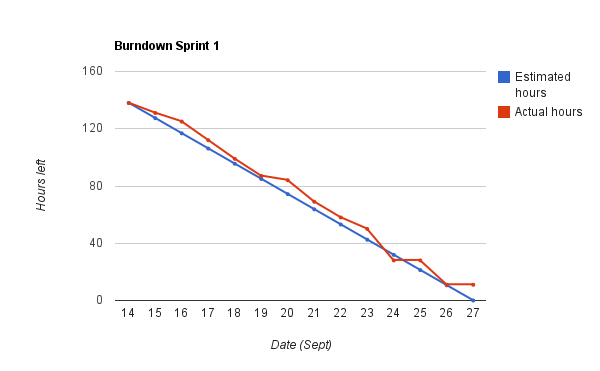
\includegraphics[width=\textwidth]{./sprints/img/burndown_chart_s1}
	\caption{Burndown chart\label{fig:sp1:burndown}}
\end{figure}

\subsection{Positive Experiences}
%--------------------------------
\begin{itemize}
	\item Good customer communication and relation from the beginning
	\item Implementation was easy
	\item Most of the requirements for this sprint were completed
	\begin{itemize} 
		\item all design, implementation and testing were completed
		\item documentation had to be putted back in the product backlog 
	\end{itemize}
	\item Errors and bugs were detected and corrected swiftly and with relative ease
	\item The team functioned well, with sufficient discussions and conflicts
\end{itemize}

\subsection{Negative Experiences}
%--------------------------------
\begin{itemize}
	\item Hard for the team members to "give" 25 person-hours each week
	\begin{itemize}
		\item to understand that it is needed
		\item to free up so many hours, and still have time to do other subjects
	\end{itemize}
	\item Hard to find time for meeting/work where all team members was able to meet
	\item One member of the team got sick
	\item We did not document the process and work during the first sprint well enough, which was a burden at the end of the sprint
	\item We did perhaps not understand scrum properly, which resulted in extra work
\end{itemize}

\subsection{Planned Actions}
%---------------------------
Below there is listed planned actions for the following sprints.

\subsubsection{Better Sprint Planning}
In order to avoid having to redo much of the work because of incorrect/poorly
sprint planning, we have decided to do this properly next time. We have learned
what we need to have in place and how to document it from this sprint.

\subsubsection{Design Early in the Sprint} 
The design should be in place early in the sprint. This is related to better
sprint planning, the planning should be so detailed/good that additional design
is not necessary. This is important for understanding and being able to
estimate hours and divide work.

\subsubsection{Documenting in Parallel while Implementing}
We suffered from the problem, code first then document. This is not a good
practise in team divided work. We will try to do the documentation as we code.
The documents for the project report also experienced a standstill while the
team worked on implementation. Writing parts of sprint documentation while
having the sprint is a much better way to work, then most part of the
documentation is already done before the sprint evaluation.

\subsubsection{Split Coding and Report Writing Between Team Members} 
Not all the team members have to do coding. It is important to maintain a
steady progress making the project report (which our grade evaluation is based
on), while doing the implementation. Responsibilities for coding and report
will be assigned next sprint. 

\subsection{Barriers}
%--------------------
Some of the team members has experience some technical difficulties with their
Git client, and others had problems setting up PyCharm. Problems rose as we
realized that there would be hard setting up the programs on different
platforms (Windows and Mac).

We had problems with C parser library, pycparser, which did not support \_Bool
type, specified in the C99 standard. A patch for this was written by Even, and
was later included in the pycparser library. There was also problems with the
testing framework, attest, this framework did not have support for Windows
command line prompt, a patch was written and was later added to their library.

Some team members had conflicting deadlines for deliveries in different courses.

